% GENERATED by scripts/srh/25_fig_dose.py -- do not edit by hand.
% Source run: results/2026-08-12_cft-bidirectional/qwen25c-1.5b/python/e3_dose_qwen1.5b
% Regenerate:
%   python scripts/srh/25_fig_dose.py --run results/2026-08-12_cft-bidirectional/qwen25c-1.5b/python/e3_dose_qwen1.5b --out paper_bidirectional/fig_dose.tex
\begin{figure}[h]
\centering
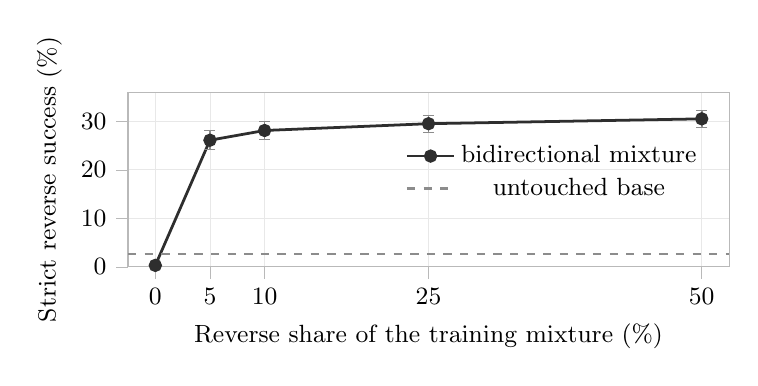
\begin{tikzpicture}
\begin{axis}[
  width=0.76\linewidth, height=3.8cm,
  xlabel={Reverse share of the training mixture (\%)},
  ylabel={Strict reverse success (\%)},
  xmin=-2.5, xmax=52.5, ymin=0, ymax=36,
  xtick={0,5,10,25,50}, ytick={0,10,20,30},
  tick align=outside, tick pos=left,
  axis line style={gray!55}, tick style={gray!55},
  grid=major, grid style={gray!18, line width=0.3pt},
  label style={font=\small}, tick label style={font=\small},
  legend style={font=\small, draw=none, fill=none, at={(0.97,0.32)},
                anchor=south east, cell picture=true},
]
\addplot[mark=*, mark size=1.9pt, line width=1pt, color=black!82,
         error bars/.cd, y dir=both, y explicit,
         error bar style={line width=0.6pt, color=black!45},
         error mark options={rotate=90, mark size=2pt, color=black!45}]
  coordinates {(0.0,0.3) +- (0,0.33) (5.0,26.1) +- (0,1.93) (10.0,28.1) +- (0,1.93) (25.0,29.5) +- (0,1.73) (50.0,30.5) +- (0,1.73)};
\addlegendentry{bidirectional mixture}
\addplot[dashed, line width=0.8pt, color=black!45, mark=none]
  coordinates {(-2.5,2.7) (52.5,2.7)};
\addlegendentry{untouched base}
\end{axis}
\end{tikzpicture}
\caption{\textbf{A little reverse data does almost all of the work.} Strict reverse
success against the reverse share of the training mixture, Qwen2.5-Coder-1.5B,
300 programs, 1\,500 graded trials per point. The zero-dose point is forward-only
SFT. Replacing just 5\% of the forward pairs with their own reverse recovers
26.1\% against 0.3\% for forward-only ---
85\%
of what a 50\% share recovers. The remaining climb is real but small
(+4.5 pp \ci{+3.2}{+5.8}
from 5\% to 50\%) and has flattened by 25\%
(+1.1 pp \ci{+0.0}{+2.1}
from 25\% to 50\%). Bars are 95\% cluster bootstraps by program; because the design is
paired, differences are quoted from the contrast table rather than read off the bars.}
\label{fig:dose}
\end{figure}
